% %--------------------
% % Packages
% % -------------------
\documentclass[11pt,a4paper]{report}
\usepackage[utf8x]{inputenc}
\usepackage[T1]{fontenc}
\usepackage[english]{babel}
\usepackage{graphicx}
\usepackage{color}
\usepackage{csquotes}
\usepackage{syntax}
\usepackage{listings, multicol}
\usepackage{subcaption}
\usepackage{tikz}
\usepackage{array}
\usepackage{enumitem}
\usepackage[compact,small]{titlesec}
\usepackage{algpseudocode}
\usepackage{algorithm}
\usepackage{url}
\usepackage{multirow}
\usepackage{breakurl}
\usepackage{amsmath}
\usepackage[hidelinks]{hyperref}
\usepackage{cleveref}
\usepackage{times}

\usepackage[
  backend=biber,
  style=numeric-comp,
  minalphanames=3,
  isbn=false,
  sortcites=true,
  sorting=anyt,
  abbreviate=false,
  url=false,
  doi=false,
  maxnames=99,
  minbibnames=3,
  maxbibnames=99]{biblatex}

\addbibresource{main.bib}

% \titleformat{\chapter}[display]
%   {\normalfont\large\bfseries}{}{0pt}{\LARGE}
% \titlespacing*{\chapter}
%   {0pt}{10pt}{20pt}

\frenchspacing
\linespread{1.2}

\newcommand{\cmt}[3]{
{\footnotesize [\textcolor{#1}{\textsf{#2: #3}}]}
}
\newcommand{\todo}[1]{
\textcolor{red}{#1}
}
\newcommand{\malte}[1]{\cmt{blue}{Malte}{#1}}
\newcommand{\justus}[1]{\cmt{olive}{Justus}{#1}}
\newcommand{\shriram}[1]{\cmt{teal}{Shriram}{#1}}
\newcommand{\livia}[1]{\cmt{red}{Livia}{#1}}
\newcommand{\carolyn}[1]{\cmt{purple}{Carolyn}{#1}}

\def\sys{\text{Para\-legal}}
\def\syslang{\text{Para\-lang\-uage}}
\newcommand{\code}[1]{{\footnotesize\texttt{#1}}}
\newcommand{\marker}[1]{\code{\color{blue}{#1}}}
\newcommand{\cnlexp}{Controlled Natural Language (CNL)}
\newcommand{\dev}{developer}
\newcommand{\devs}{developers}
\newcommand{\Devs}{Developers}
\newcommand{\policies}{privacy policies}
\newcommand{\writer}{\ce}
\newcommand{\writers}{\ces}
\newcommand{\Writers}{\Ces}
\newcommand{\ce}{compliance engineer}
\newcommand{\ces}{compliance engineers}
\newcommand{\Ce}{Compliance engineer}
\newcommand{\Ces}{Compliance engineers}
\newcommand{\policylang}{privacy policy specification language}
\newcommand{\controller}{entrypoint}
\newcommand{\Controller}{Entrypoint}

\lstdefinelanguage{Rust}{%
    morekeywords={impl,let,in,return,fn,struct,enum,mut,for,region,where,if,else,pub,use},
    sensitive=true,
    otherkeywords={{->}, {=}, {|}, {:}, {.}, {&}, {?}},
    morecomment=[l]{//},
    morecomment=[s]{/*}{*/},
    morestring=[b]",
    morestring=[d]',
}
\lstdefinelanguage{CNL}{
  morestring=[b]",
  stringstyle=\color{violet},
  moredelim={[is][\color{teal}]{@@}{@@}},
  moredelim={[is][\color{blue}]{/*}{*/}}
}

\lstset{
    language=Rust,
    basicstyle=\ttfamily\footnotesize,
    columns=fullflexible,
    keepspaces=true,
    showspaces=false,
    showstringspaces=false,
    showtabs=false,
}

\setlist{leftmargin=*}

\setlength{\fboxsep}{1pt}%

\begin{document}

\lstMakeShortInline|

\thispagestyle{empty}

\begin{center}
    \vspace*{1em}{\Huge \syslang{}: A Privacy Policy Specification Language \par}
    
    \vspace*{1em}{\huge Carolyn Zech\par}
    
    \vspace*{3em}{\LARGE Advisor: Malte Schwarzkopf\par Reader: Shriram Krishnamurthi\par}
    
    \vspace*{8em}
\includegraphics[scale=0.08]{graphics/logo.png}\par
    \vspace*{1em}{\LARGE Department of Computer Science\par Brown University\par Providence, RI \par May 2024 \par}
\end{center}
\newpage

\tableofcontents
\newpage

\section*{Abstract}

%
Software providers handling sensitive data must verify that their applications conform to a wide breadth of \policies.
%
For example, to comply with the GDPR, providers must check that their applications contain logic to delete all of a user's personal data.
% 
Existing tools to express \policies{} are either expressive but overly technical, or are nontechnical but also not expressive.
%
\syslang{} is a new \policylang{} that is both expressive and accessible to nontechnical stakeholders.
%
\syslang{} can specify a wide range of \policies{} in an intuitive, natural language format.
%
Our \syslang{} compiler outputs graph queries over a program dependence graph (PDG),
which developers can then run against their applications to verify compliance.
%
We evaluate \syslang{} on seven real-world Rust applications and find that it is
sufficiently expressive, precise, and efficient.
\carolyn{some actual hard data would be nice here -- come back after eval is fleshed out}
% \section*{Acknowledgments}
\addcontentsline{toc}{section}{Acknowledgments}
\chapter{Introduction}
\label{sec:intro}

Privacy bugs in applications harm users (e.g., by leaking their sensitive data) and put software providers 
at risk for financial liability.
%
In May of 2023 alone, Ireland fined Meta €1.2 billion for GDPR violations, 
while the United States fined Amazon \$25 million for failing to honor data deletion requests 
under the Children’s Online Privacy Protection Act~\cite{meta-fine,amazon-fine}.
%
To ensure compliance, organizations must relate dense legal text to their low-level application source code.
%
Currently, organizations use manual audits to verify compliance, which are expensive, time-consuming,
and infrequent~\cite{CostContinuousCompliance2020,smithGDPRRacketWho}.
%

\sys{} is a static analyzer for Rust applications that \devs{} leverage to find such bugs in their programs before deployment.
%
\sys{} evaluates an application by generating its program dependence graph (PDG), 
where nodes are program entities (arguments, types, etc.) and edges are control or data flow dependencies.
%
\sys{} evaluates the PDG against the policy and outputs whether the application is compliant.

\Devs{} can receive immediate feedback on the impact of their changes by running 
\sys{} continually throughout the development process, perhaps as part of a CI pipeline.
%
We envision that \sys{} could replace (or at least reduce the frequency of) manual compliance audits.


\section{The Problem}
\sys{} policies are Rust programs that execute low-level graph queries over an application's PDG.
%
To write these programs, \devs{} must first connect high-level concepts 
(e.g., ``all sensitive data is encrypted'')
to low-level implementation details.
%
They must then understand how \sys{} represents these details with a PDG,
and finally translate their high level policy into a series of assertions about paths in this graph.
%
This design limits the available pool of policy writers to those with 
an in-depth understanding of Rust programming, application semantics, and \sys{}'s PDG representation.
%
Since policies are programs, they have the same problems as the applications they evaluate: 
they are buggy, laborious to write, and comprehensible only to programmers familiar with the application.

Ideally, policy writers would specify only the high-level concepts behind their policy,
which \sys{} would translate automatically into an application-specific query.
%
We realize this goal with \syslang{}, a DSL for \policies{} over PDGs.
%
\syslang{} is a Controlled Natural Language (CNL) interface; users write policies in natural language, 
but are restricted to a defined grammar ~\cite{cnl-def}.
%
Natural language offers the intuitive quality we seek, 
while the grammar allows us to avoid the ambiguity of unconstrained English.
%
We pair \syslang{} with a compiler that translates policies to \sys{} graph queries in Rust.
%
\Devs{} then invoke \sys{} on their application,
which generates its PDG, evaluates it against the compiled \syslang{} policy,
and outputs whether the application is compliant.
%

\section{Goals}
The design of \syslang{} must address four challenges.

First, it must be accessible yet unambiguous.
%
\syslang{} should avoid requiring policy writers to reason about low-level source code entities, 
such as particular functions or arguments.
%
Such a design would tie the policy to the application's implementation, 
effectively restricting policy writing to the application's \devs.
%
It would also make the policies more difficult to write and brittle to source code changes.
%
\syslang{} should instead be accessible to a range of technical stakeholders.
%
Ideally, a \ce--someone who knows how to program, 
but who is not necessarily familiar with the particular implementation details--would write policies in a code-agnostic way.
%

Natural language provides an intuitive structure for specifying these policies.
%
However, unconstrained natural language can be ambiguous.
%
For example, the sentence ``|A| or |B| and |C|'' is vague; which operator should take higher precedence?
%
While such ambiguity may be acceptable (or even desirable) in legal text,
it is unacceptable for a policy that is checkable by an automated tool.
%
\syslang{} must reject ambiguous policies without becoming so onerous to use that it 
requires the same expertise and time investment as writing a graph query program.

Second, \syslang{} should be expressive.
%
A trivial way of eliminating ambiguity would be to define a highly restricted natural language interface that allows for only a handful of policy formulations.
%
This structure, however, would be insufficiently expressive to meet the needs of complex applications, 
which must abide by a wide range of privacy requirements.
%
Instead, \syslang{} should be flexible enough to apply across policy and application domains.

Third, \syslang{} should support sufficiently precise queries to express common \policies{}, 
without overwhelming the \writer{} with the specifics of \sys{}'s PDG representation. 
%
\sys{}'s PDG representation represents program structure with a specific level of precision.
%
With the existing graph query interface, \writers{} can leverage this precision to make highly specific queries
(e.g., count the exact number edges between two nodes in a graph). 
%
However, \policies{} often do not require this level of precision.
%
If \syslang{} were to require reasoning about the PDG specifics, 
it would not be accessible--\ces{} would require expertise
to choose from a wide array of query patterns over a complex, unfamiliar data structure.
%
However, if policies are insufficiently precise, they are more likely to produce false positives or false negatives when run against application code.

Fourth, \syslang{} policies, once compiled, should be similarly efficient to graph queries written in Rust.
%
This goal is necessary so that \sys{} runs at interactive timescales when checking \syslang{} policies.

We evaluate \syslang{} against seven third-party Rust applications.
%
We find that \syslang{} can express a wide range of \policies{} for these applications,
that these policies correctly identify bugs,
and that they incur acceptable run time overhead ($\approx$0-12\%) compared to hand-optimized Rust graph queries.

\bigskip{}
\emph{\sys{} is the product of collaboration with Justus Adam, Livia Zhu, Sreshtaa Rajesh, 
Will Crichton, Shriram Krishnamurthi, and Malte Schwarzkopf.
My contribution specifically is the \syslang{} policy language and the compilation to Rust policies.}

\section{Background}

% brief "this is what paralegal is" -- \controller{}s, PDGs, etc.
% pdgs are per \controller{}
% may be able to shove necessary background knowledge into overview,
% but may be good to do it ahead of time so as to not distract from the example

\chapter{Overview}
\label{sec:overview}

\Ces{} and \devs{} collaborate to apply \sys{} to their applications and catch privacy bugs before deployment.
%
We demonstrate \syslang's role in this process through an example.

Freedit is a text-based social media application, similar to Reddit or Twitter~\cite{freedit}.
%
The application stores a user's viewing history, but deletes it after three days~\cite{freedit-pageviews}.
%
To verify that the source code upholds the policy, 
a \ce{} must first ensure that any viewing data is always stored alongside the current date.
%
Otherwise, the application would have no way to check later whether the data is expired.
%
To encode this policy in \syslang{}, the \ce{} first considers which operations or data are relevant to the policy.
%
They determine that the relevant concepts for this policy are \emph{(i)} the viewing data,
\emph{(ii)} any database store operations, and \emph{(iii)} the current date.
%
They define \lstinline[language=CNL]|@@views@@|, 
\lstinline[language=CNL]|@@store@@|, 
and \lstinline[language=CNL]|@@time@@| markers to represent each of these ideas.
%
The \ce{} must have some technical background to establish these concepts--they must, for example, understand what a database is,
and the kind of data that it would store.
%
However, they do not need to understand how the source code implements this functionality,
or the details of the database client library that the app uses.
%

Next, the \ce{} writes the policy in terms of these markers.
%
They know that a \dev{} will eventually apply their markers to one or more source code entities.
%
Their policy must therefore reason about these marked object(s).
%
To do so, the \ce{} introduces \emph{variables} into their policy.
%
A variable represents a single source code entity with a given marker.
%
In this example, the \ce{} introduces their variables as follows:
\begin{lstlisting}[language=CNL]
For each "view" marked @@views@@:
  For each "database store" marked @@store@@:
\end{lstlisting}
%
Here, and in the following text, variables are in purple and markers are in teal.

The \ce{} must now establish that a given \lstinline[language=CNL]|"database store"| actually stores this \lstinline[language=CNL]|"view"|--
if it stores some other, unrelated data, the policy does not apply.
%
To do so, they introduce the first \emph{predicate} into their policy:
\begin{lstlisting}[language=CNL]
For each "view" marked @@views@@:
  For each "database store" marked @@store@@:
    /*If*/ "view" /*goes to*/ "database store" /*then:*/
\end{lstlisting}
%
Predicates are expressions that relate two objects to each other--either two variables, or a variable and a marker.

Note that the \ce{} need not specify \emph{how} or \emph{when} the \lstinline[language=CNL]|"view"| reaches the \lstinline[language=CNL]|"database store"|.
%
The \lstinline[language=CNL]|"view"| could undergo any number of data transformations first--e.g., it could be inserted as a field of a type containing other user data,
and that type is then stored.
%
The \ce{} does not worry about these implementation details; they must only understand that the \lstinline[language=CNL]|"view"| reaches the \lstinline[language=CNL]|"database store"|
in some form, at some point.
%

The \ce{} then defines the consequent of the conditional:
\begin{lstlisting}[language=CNL]
For each "view" marked @@views@@:
  For each "database store" marked @@store@@:
    If "view" goes to "database store" then:
      /*There is a*/ "date" /*marked*/ @@time@@ /*where:*/
        "date" /*goes to*/ "database store"
\end{lstlisting}
%
The consequent ensures that if the view is stored, that some date is also stored.
%
% Since both the antecedent and the consequent reason about the same \lstinline[language=CNL]|"database store"| variable,
% the \ce{} ensures that the date and view are stored \emph{together}.
%
% Without variables, the \ce{} could only write that the current date goes to some entity marked \lstinline[language=CNL]|@@store@@|,
% but this could be a completely different store unrelated to \lstinline[language=CNL]|"view"|.

Finally, the \ce{} establishes the \emph{scope} of their policy,
%
For instance, a GDPR data deletion policy would assert that somewhere in the application, 
all of a user's data is deleted.
%
In this case, the \ce{} determines that the entire application should uphold this policy, so they select the ``Everywhere'' scope,
producing the final policy:

\begin{lstlisting}[language=CNL]
/*Scope: Everywhere*/

/*Policy:*/
For each "view" marked @@views@@:
  For each "database store" marked @@store@@:
    If "view" goes to "database store" then:
      There is a "date" marked @@time@@ where:
        "date" goes to "database store"
\end{lstlisting}

The \ce{} then sends this policy to a \dev{}, 
who leverages their implementation knowledge to apply the markers to the appropriate source code entities.
%
Here, they might attach the \lstinline[language=CNL]|@@views@@| marker on all function arguments of type |PageView|,
the \lstinline[language=CNL]|@@store@@| marker on an argument to a database library insertion function,
and the \lstinline[language=CNL]|@@time@@| marker on the return value of a function that gets the current date.
%
The \dev{} runs \syslang{}'s compiler, 
which outputs a Rust program that contains an equivalent graph query over a marked PDG 
and boilerplate code to invoke \sys{}.
%
\sys{} generates the application's marked PDG, 
evaluates it against the policy,
and outputs whether the policy passed or failed.
%

\chapter{Design}
\label{sec:design}

\syslang{} is comprised of two components: its surface language in which \ces{} write policies,
and its compiler that translates those policies to graph queries over a marked PDG.

\section{Surface Language}
\label{sec:interface}

A \syslang{} policy has two to three sections: its scope, (optionally) its definitions, and its body.

\subsection{Scope}
\label{sec:scope}

A \ce{} has three options for the scope of their policy:
%
\begin{enumerate}[nosep]
    \item \emph{Everywhere} indicates that every \controller{} should obey the policy.
    \item \emph{Somewhere} indicates that at least one \controller{} should obey the policy.
    \item \emph{In} |name| indicates that the \controller{} with name |name| should obey the policy.
\end{enumerate}

The appropriate scope is policy-dependent.
%
For instance, if an application should always encrypt sensitive data before storage,
the \ce{} should select an ``Everywhere'' scope.
%
For a GDPR data deletion policy, however, an ``Everywhere'' scope would not make sense, 
since that would require every \controller{} storing user data to also delete it.
%
Instead, such a policy could use a ``Somewhere'' scope to mandate that at least one \controller{} deletes user data.
%
\Ces{} may wish to be more specific and ensure that a particular \controller{} deletes user data as specified,
in which case they should use the \emph{In} |name| scope.
%
This scope achieves greater precision, but is also tied to the source code; if the name of the data deletion \controller{} changes, the policy must change as well.
%

\subsection{Definitions}
\label{sec:definitions}

In the Freedit example from \S\ref{sec:overview}, the \ce{}'s final policy was:
\begin{lstlisting}[language=CNL]
For each "view" marked @@views@@:
  For each "database store" marked @@store@@:
    If "view" goes to "database store" then:
      There is a "date" marked @@time@@ where:
        "date" goes to "database store"
\end{lstlisting}
This policy contains five levels of nesting.
%
As policies get more complex, many levels of nesting can make policies inefficient and harder to understand.
%
To address this issue, \syslang{} allows \ces{} to create \emph{definitions}.
%
A definition defines a variable ahead of time which refers to all nodes in a given \controller{}'s PDG that meet a certain condition.
%
Observe that the Freedit policy does not enforce any obligations on a \lstinline[language=CNL]|"database store"| unless it stores a \lstinline[language=CNL]|"view"|.
%
Rather than iterate through \emph{all} database stores, 
a \writer{} can collect only the relevant database stores up front,
then write their policy in terms of those.
%
In this case, the Freedit \ce{} would create the following definition:
\begin{lstlisting}[language=CNL]
"view store" is each "store" marked @@db_store@@ where:
  There is a "view" marked @@views@@ where:
    "view" goes to "store"
\end{lstlisting}
and revise their policy to:
\begin{lstlisting}[language=CNL]
For each "view store":
  There is a "date" marked time where:
    "date" goes to "view store" 
\end{lstlisting}
This policy is also more efficient because it avoids the double ``for each'' loop of the original,
which may be expensive in an application that has many \lstinline[language=CNL]|"view"|s or \lstinline[language=CNL]|"database store"|s.
%

Since \sys{} constructs per-\controller{} PDGs,
\syslang{} policies, once compiled, are evaluated against one \controller{} at a time.
%
The scope of the policy dictates which \controller{}(s) must uphold the policy.
%
Since policy bodies only consider nodes in the current \controller{}'s PDGs,
definitions are also, by default, \controller{}-specific

By default, definitions are also evaluated on a per-\controller{} basis.
%
However, a \ce{} may want to gather all nodes meeting a certain condition \emph{across \controller{}s}.
%
For instance, consider a policy that states that for each |sensitive| type that the application |store|s,
that type is also |delete|d.
%
It is unlikely that a single \controller{} would both store the sensitive data \emph{and} delete it.
%
Instead, the \ce{} could declare a definition to gather the relevant types from across the application,
then write a policy that states that some \controller{} must delete those types.
%
They would do so by appending ``anywhere in the application'' to their definition declaration,

% Such a policy would look like the following:
% \begin{figure}[h]
% \begin{lstlisting}[language=CNL]
% Scope: Somewhere

% Definitions:
% "stored sensitive" is each "sensitive" type marked @@sensitive@@ where, 
% anywhere in the application:
%     There is "database store" marked @@store@@ where:
%       "sensitive" goes to "database store"

% Policy:
% For each "stored sensitive":
%     There is a "deleter" marked @@deletes@@ where:
%       "stored sensitive" goes to "deleter"
% \end{lstlisting}
% \end{figure}

\begin{figure}[t]
    \small
    \begin{tabular}{|p{5.5cm}|p{8cm}|}
        \hline
        \syslang{} Relation                                                       &  Obligation on PDG                   \\ \hline
        \lstinline[language=CNL]|"a" goes to "b"|                                 &  There is some transitive data flow dependency from
                                                                                    \lstinline[language=CNL]|"a"| to \lstinline[language=CNL]|"b"|. \\
        \hline
        \lstinline[language=CNL]|"a" affects whether "b" happens|                 & There is some transitive control flow dependency from
                                                                                    \lstinline[language=CNL]|"a"| to \lstinline[language=CNL]|"b"|. \\
        
        \hline
        \lstinline[language=CNL]|"a" goes to "b" only via "c"|                    &  On every data path from \lstinline[language=CNL]|"a"| to \lstinline[language=CNL]|"b"|,
                                                                                    \lstinline[language=CNL]|"a"| passes through \lstinline[language=CNL]|"c"|. \\
        \hline
        \lstinline[language=CNL]|"a" influences "b"|                              &  There is some transitive data flow and/or control flow dependency from  \lstinline[language=CNL]|"a"| to \lstinline[language=CNL]|"b"|.  \\
        \hline
        \lstinline[language=CNL]|"a" is marked @@m@@|                             & \lstinline[language=CNL]|"a"| is marked \lstinline[language=CNL]|@@m@@|. \\
        \hline
        \lstinline[language=CNL]|"a" goes to "b"'s operation|                     & \lstinline[language=CNL]|"a"| goes to the call site associated with \lstinline[language=CNL]|"b"|,
                                                                                    e.g., if \lstinline[language=CNL]|"b"| is an argument to a call site, then \lstinline[language=CNL]|"a"| goes to any of that call site's arguments or return. \\        
      \hline
    \end{tabular}
      \caption{\syslang's relations and the obligations they enforce on \sys's marked PDG.}
      \label{f:relations}
  \end{figure}

\subsubsection{Body}
\label{sec:body}

The policy body has three components: iterators, relations, and conjunctions/disjunctions of them.
%
\paragraph{Iterators}
Iterators allow \ces{} to loop over a collection of nodes, reasoning about one node at a time.
%
\syslang{} provides two iterators: a ``For each'' loop or a ``There is'' statement.
%
To iterate over a defined variable \lstinline[language=CNL]|"x"|, 
a \ce{} would write \lstinline[language=CNL]|For each "x" marked @@m@@:| or \lstinline[language=CNL]|There is a "x" marked @@m@@ where:|
%
To introduce a new variable,
a \ce{} would write \lstinline[language=CNL]|For each "x" marked @@m@@:| or \lstinline[language=CNL]|There is a "x" marked @@m@@ where:|
%
A ``For each'' loop iterates over each object in the collection and evaluates the body of the loop 
in the context of the current object \lstinline[language=CNL]|"x"|.
%
It succeeds if the body is true for all \lstinline[language=CNL]|"x"|.
%
If there are no objects in the collection, the policy is vacuously true.
%
\syslang{} allows for vacuity because it evaluates policies on a per-\controller{} basis,
and some \controller{}s may not have certain markers.
%
For example, take the Freedit policy from \S\ref{sec:overview}:
\begin{lstlisting}[language=CNL]
Scope: Everywhere

Policy:
For each "view" marked @@views@@:
  For each "database store" marked @@store@@:
    If "view" goes to "database store" then:
      There is a "date" marked @@time@@ where:
        "date" goes to "database store"
\end{lstlisting}

Since the policy's scope is ``Everywhere'', it will be evaluated against every \controller{},
regardless of whether it handles view data.
%
It would be confusing for a \dev{} if their application failed the policy on a \controller{} 
that does not even contain the \lstinline[language=CNL]|@@views@@|.
%
The \ce{} could avoid this problem by changing their scope to list every \controller{} to which they expect the policy to apply,
but that would defeat \syslang's goal of being independent from source code.
%
If the \ce{} wants to insert such a vacuity check, they can leverage the ``There is'' iterator, like so:
\begin{lstlisting}[language=CNL]
  Scope: Everywhere
  
  Policy:
  There is a "view" marked @@views@@ where:
    There is a "database store" marked @@store@@ where:
      "view" goes to "database store"
  and
  For each "view" marked @@views@@:
    For each "database store" marked @@store@@:
      If "view" goes to "database store" then:
        There is a "date" marked @@time@@ where:
          "date" goes to "database store"
\end{lstlisting}
%
The ``There is'' iterator succeeds if the body is true for at least one \lstinline[language=CNL]|"x"|.
%
If there are no objects in the collection, the policy is false.
%
Observe that the loop bodies reason about the iterator variables.
%
If instead, we eschewed iterators and wrote this policy as:
\begin{lstlisting}[language=CNL]
If "view" goes to a "database store" marked @@store@@:
  There is a "date" marked @@time@@ where:
    "date" goes to a "database store" marked @@store@@
\end{lstlisting}
We would not enforce that \lstinline[language=CNL]|"view"| and \lstinline[language=CNL]|"date"| 
go to the \emph{same} \lstinline[language=CNL]|"database store"|.
%
This policy, however, would pass as long as the date is stored anywhere else in the application,
even if it is in a context completely unrelated to views.
%
Iterators enable for the correct version of the policy by allowing \ces{} to refer to the same object multiple times.

\paragraph{Relations}
%
Relations are between two objects: either two variables and a variable and a marker.
%
The full list of available relations are in Figure~\ref{f:relations}.
%
\syslang{} also supports the negation of each of these relations, e.g. \lstinline[language=CNL]|"a" does not go to "b"|.
%
\Ces{} use |and| or |or| operators to join iterators or relations together.

\Ces{} also need to indicate the scope of each iterator.
%
In our examples thus far, we have used indentation to nest iterators.
%
However, such a design is error-prone--one accidental indentation, and a \ce{} compiles an entirely different policy than what they intended.
%
For instance, take the policies in Figure~\ref{f:indentation}, which differ only in indentation but have different meanings.
%
Version (1) will only enforce that the sensitive value is encrypted if it is stored.
%
Version (2) enforces that the sensitive value is encrypted regardless.

\begin{figure}[t]
    \begin{subfigure}[b]{\columnwidth}
  \begin{lstlisting}[language=CNL]
    If "sensitive" goes to "store" then:
      "sensitive" goes to "auth check"
      and
      "sensitive" goes to "encrypts"
  \end{lstlisting}
  \caption{Version 1 of the policy.}
  \end{subfigure}
  \begin{subfigure}[b]{\columnwidth}
  \begin{lstlisting}[language=CNL]
    If "sensitive" goes to "store" then:
      "sensitive" goes to "auth check"
    and
    "sensitive" goes to "encrypts"
    \end{lstlisting}
    \caption{Version 2 of the policy.}
    \end{subfigure}
    \caption{Two policies with identical syntax but different scopes. These policies are partial; we elide iterator declarations for brevity.}
    \label{f:indentation}
\end{figure}

\begin{figure}[t]
    \begin{subfigure}[b]{\columnwidth}
  \begin{lstlisting}[language=CNL]
    1. If "sensitive" goes to "store" then:
      A. "sensitive" goes to "auth check"
      and
      B. "sensitive" goes to "encrypts"
  \end{lstlisting}
  \caption{Version 1 of the policy.}
  \end{subfigure}
  \begin{subfigure}[b]{\columnwidth}
  \begin{lstlisting}[language=CNL]
    1. If "sensitive" goes to "store" then:
      A. "sensitive" goes to "auth check"
    and
    2. "sensitive" goes to "encrypts"
    \end{lstlisting}
    \caption{Version 2 of the policy.}
    \end{subfigure}
    \caption{The policies from Figure~\ref{f:indentation} with bullets to explicitly delineate each expressions's scope.}
    \label{f:bullets}
\end{figure}

Rather than allow a stray indent to change the meaning of the policy,
\syslang{} instead enforces that \ces{} explicitly specify the scope of each statement.
%
They do so using \emph{bullets}.
%
Figure~\ref{f:bullets} shows the policies from Figure~\ref{f:indentation} with \syslang{} bullets.
%
\Ces{} are not permitted to mix operators (|and|s and |or|s) on the same bullet level,
since the operator precedence in such cases would be ambiguous.

\syslang{}'s full grammar is in \Cref{sec:grammar}.

\section{Compiler}

The \syslang{} compiler translates policies into graph queries over \sys{}'s PDG,
which \devs{} run against their application.
%
The compiler first parses the policy into an abstract syntax tree (AST).
%
It then traverses this AST to verify that the policy is properly scoped.
%
It errors if any variables are used in a relation without first being introduced by an iterator or definition.
%
It also prohibits duplicate introductions of the same variable in the same scope.

Once the compiler verifies that the policy is properly scoped,
it performs a second pass over the AST to compile it to Rust code.
%
It performs compilation via template expansion.
%
It identifies the relevant template for each node in the AST,
substituting in the policy's variables and markers.
%
The |and|, |or|, |for each|, |there is|, and |if| constructs correspond directly to Rust builtin operators.
%
Relations compile to expressions using \sys{}'s Graph Query API.
%
For example, \lstinline[language=CNL]|"x" goes to "y"| compiles to |flows_to(x, y, EdgeSelection::Data)|.
%
The compiler outputs a binary file containing the policy.
%
This binary contains boilerplate code to invoke \sys{} against the policy,
which the \dev{} edits to provide application-specific information,
such as the application directory
and optional \sys{} configuration flags.
%


\chapter{Implementation}

We implement the \syslang{} compiler in 2370 lines of Rust.

\syslang{} has some limitations which could be overcome with further engineering effort.
%
We detail those below.

\section{Direct Dependencies}
\label{sec:direct-limits}
\syslang{} relations reason about \emph{transitive} dependencies between PDG nodes.
%
There is no way for \ces{} to enforce a \emph{direct} edge between two nodes.
%
In most cases, transitive dependencies are the correct level of abstraction.
%
For example, given the code \lstinline[language=Rust]|sink(*sensitive)|,
one would reasonably conclude that |sensitive| goes to |sink|.
%
However, since |sensitive| is dereferenced, the PDG would contain an intermediate node between |sensitive| and |sink|,
so there is no direct data flow edge between |sensitive| and |sink|.
% \carolyn{Double check with Justus that this dereference example works; otherwise, introduce a toy example where sensitive flows to an intermediate variable,
% which then flows to sink.}
%
However, it is possible that a \dev{} would want to forbid any intermediate data transformations
to sensitive data before it reaches some |sink| (perhaps in a security-critical setting).
%
\syslang{} could not express this policy, while \sys{}'s Graph Query API can.

\section{Code Improvements}
\label{sec:code-limits}
The \syslang{} compiler does not optimize its outputted code, so it misses opportunities for efficiency improvements.
%
For example, if a policy contains two iterators over the same data, the \syslang{} compiled policy will traverse the PDG twice,
when it could have just done one traversal and stored the result for the subsequent iteration.

The Graph Query API also has a sophisticated error messages framework,
which allows \devs{} to print which source code locations are causing policy failure.
%
\syslang{}'s policies currently only print whether the policy was successful,
but the compiler's templates could be revised to support this error message framework.
%

\section{Other Limitations}
\label{sec:other-limits}
Our \syslang{} prototype supports five levels of bullets, but more could be added with additional engineering effort.
%
It also only supports iterating over defined variables and variables marked \lstinline[language=CNL]|@@m@@|.
%
If \syslang{} allowed filtering on relations, e.g. \lstinline[language=CNL]|For each "x" that goes to "y"|,
its policies would be more concise.

\chapter{Evaluation}

\begin{figure*}
    \centering
    \small
     \begin{tabular}{l|c|r|l}
       \bf Application        & \bf Type    & \bf LoC & \bf Policies   \\
      \hline
       Atomic~\cite{atomic} (v0.34.2)       & Graph DB    & 9.6k   & Access Control                                 \\
       Contile~\cite{contile} (v1.11.0)     & Advertising & 4.9k     & Purpose Limitation                           \\
       Freedit~\cite{freedit} (v0.6.0-rc.3) & Social      & 6.6k     & Data Retention/Expiration                     \\
       Hyperswitch~\cite{hyperswitch} (v0.2.0)   & Payments    & 198.9k     & Credential Security, Limited Data Collection  \\
       Lemmy~\cite{lemmy} (v0.16.6)        & Social      & 31.4k   & Access Control                               \\
       Plume~\cite{plume} (v0.7.2)         & Blogging    & 21.4k   & Data Deletion                                \\
       WebSubmit~\cite{websubmit} (v1.0)       & Homework    & 1.6k    & Data Deletion, Access Control     \\
    \end{tabular}
    \caption{Case study applications with code size and policies.}
    \label{f:apps}
   \end{figure*}

We evaluate \syslang{} against seven third-party Rust applications to answer four questions:
%
\begin{enumerate}[nosep]
    \item What is the developer effort required to encode policies in \syslang? (\S\ref{sec:accessibility})
    \item Can \syslang's grammar express real-world \policies? (\S\ref{sec:expressivity})
    \item Does \syslang's compiler correctly translate \policies{} to graph queries without loss of precision? (\S\ref{sec:precision})
    \item Does \syslang's compiler produce efficient, optimized queries? (\S\ref{sec:efficiency})
\end{enumerate}
%

We tried to pick popular applications spanning different policy domains.
%
We summarize the applications in~\Cref{f:apps}.

\section{Developer Effort}
\label{sec:accessibility}
%
We evaluate the effort required to encode policies in \syslang{}.
%
One of \syslang's goals is to be accessible and intuitive to \ces{} without advanced programming experience or implementation knowledge.
%
For each application, we had two groups write policies.
%
The first group wrote the policies using the Graph Query API, while the other used \syslang{}.
%
The Graph Query API group simulated the process of an application \dev{} who decided on policies by referencing application source code.
%
The \syslang{} group emulated the role of a \ce{}.
%
They did not look at source code, but rather used demo applications and documentation to determine their policies.
%
Ideally, we would have conducted this experiment with users unfamiliar with \sys{}.
%
However, the results still serve as a useful relative comparison between the two forms of policy writing,
even if they cannot speak to their absolute ease of use.

We found that the \syslang{} policies were easier to write and required less debugging.
%
The Graph Query API policies were tied closely to the source code and used more markers than the \syslang{} policies.
%
They were also 2-3$\times$ longer than the \syslang{} policies, 
which made it harder to understand what they were doing and identify bugs.


\section{Expressivity}
\label{sec:expressivity}
%
We found that \sys{} could express all of the policies of these applications.
%
In cases where the policy was inherently dynamic, we defined static approximations.
%
For example, a GDPR data deletion policy would state that some \controller{} deletes \emph{all} of a user's data.
%
\sys{} cannot verify that the application actually deletes all of the user's data,
since the exact contents of that data is only known at runtime.
%
However, it can ensure that for each type marked \lstinline[language=CNL]|user_data|, 
there is some data of that type that goes to a \lstinline[language=CNL]|deleter|.
%
This policy is expressive enough to find bugs where applications forget to delete a given type of user data,
but cannot catch bugs where an application only deletes \emph{some} of the data of a given type.
%
We also found that applications could often use identical policies.
%
For instance, two applications (mCaptcha and Plume) use the same data deletion policy.
%
Three others (Hyperswitch, Lemmy, and mCaptcha) use the same access control policy
except for application-specific markers.
%

\section{Precision}
\label{sec:precision}
\syslang{} policies do not support the same degree of precision as native Rust polices~\Cref{sec:interface,sec:limitations}.
%
We evaluate to what extent this loss of precision affects the accuracy of \syslang{} policies.
%
We ran both the Graph Query API policies and the \syslang{} policies on compliant versions of the applications and 
versions with injected bugs.
%
We found that the policies produced identical results, 
i.e., a \dev{} would catch the same bugs (and have the same false positives) with either version.
%

While this result is a promising indicator that \syslang's worse precision is acceptable in practice,
there are cases where it would miss bugs that a Graph Query API policy could catch.
%
For example, take the function |send_email(recipient, sender, content)|.
%
A \ce{} may want to enforce that if \lstinline[language=CNL]|@@sensitive@@| data is sent,
the recipient is an administrator.
%
However, if the \ce{} simply checked that data marked \lstinline[language=CNL]|@@admin@@| goes to \emph{some} |recipient|,
then code like this would pass the policy:
\begin{lstlisting}[language=Rust]
    send_email(admin@cs.brown.edu, student1@cs.brown.edu, benign_data);
    send_email(student1@cs.brown.edu, student2@cs.brown.edu, sensitive_data);
\end{lstlisting}
The second |send_email| call is unsafe because sensitive data is sent to a student, not an administrator.
%
However, because the first, unrelated |send_email| recipient is an administrator, \sys{} would see that some recipient is an admin and the policy would pass.
%
To prevent this bug, a \ce{} could make their policy more precise, and instead say that if data marked \lstinline[language=CNL]|@@sensitive@@| goes to |content|,
then data marked \lstinline[language=CNL]|@@admin@@| goes to |recipient| \emph{in the same} |send_email| \emph{operation}.
%
\syslang{} cannot express this policy exactly.
%
It can get close--it can express that data marked \lstinline[language=CNL]|@@admin@@| goes to the same operation,
but it cannot enforce that it goes to the |recipient| argument specifically.
%
Thus, the \syslang{} version of the policy would allow this (buggy) code to pass:
\begin{lstlisting}[language=Rust]
    send_email(student1@cs.brown.edu, student2@cs.brown.edu, 
                "admin@cs.brown.edu's SSN is [...]");
\end{lstlisting}
%
\sys{}'s Graph Query API can enforce that the administrator goes to the correct argument,
so it is possible to write a native Rust policy that catches this bug.

\section{Efficiency}
\label{sec:efficiency}
For each application, we compare the total execution time of its Graph Query API policies
and their \syslang{} policies.
%
To avoid the variance of a single run unduly affecting the result, we average the results over 10 runs each.
%
We would expect \syslang{} policies to be slower on average because of its compiler limitations (\S\ref{sec:limitations}).
%
We found that \syslang{} policies are 2-12\% slower than their Graph Query API counterparts.
%
The one exception is WebSubmit, which was 0.5\% faster than the Rust API policies.
%
However, the WebSubmit policies run quickly (~25-30ms for 3 policies),
so in any given run, this percentage varies widely.
%
Figure~\ref{f:times} compares the \syslang{} execution times to the Graph Query API execution times.
%
\begin{figure}
    \begin{centering}
        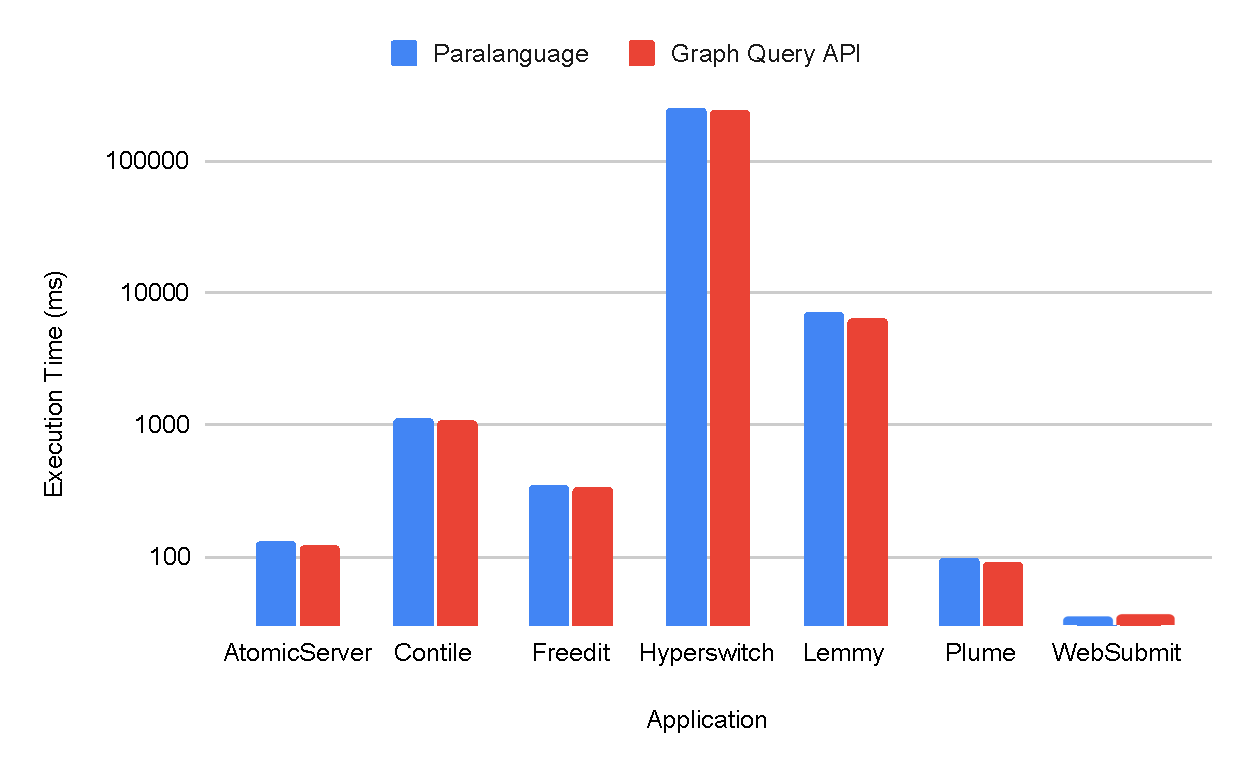
\includegraphics[scale=0.7]{graphics/times.pdf}
        \caption{\syslang{} and Graph Query policy execution times, averaged across 10 runs.}
        \label{f:times}
    \end{centering}
\end{figure}
%
Figure~\ref{f:percentages} gives the percentage difference in run time for each application.
\begin{figure}
    \begin{tabular}{|l|p{3cm}|p{3.5cm}|p{2cm}|p{3cm}|}
        \hline
        \textbf{Application} & \textbf{\syslang{} Time (ms)} & \textbf{Graph Query API Time (ms)} & \textbf{Difference (ms)} & \textbf{\syslang{} \% Slower} \\ \hline
        AtomicServer & 127.92    & 118.8     & 9.12    & 7.68  \\ \hline
        Contile      & 1109.14   & 1064.43   & 44.71   & 4.2   \\ \hline
        Freedit      & 347.57    & 339.85    & 7.72    & 2.27  \\ \hline
        Hyperswitch  & 251044.37 & 241890.42 & 9153.95 & 3.78  \\ \hline
        Lemmy        & 7026.23   & 6277.3    & 748.93  & 11.93 \\ \hline
        Plume        & 95.63     & 88.86     & 6.77    & 7.62  \\ \hline
        WebSubmit    & 29.89     & 30.07     & -0.18   & -0.6  \\ \hline               
        \end{tabular}
        \caption{Comparison of \syslang{} and Graph Query API policy execution times.}
        \label{f:percentages}
\end{figure}
%
These results demonstrate that \syslang{} policies incur an acceptable overhead compared to native Rust policies.

\chapter{Related Work}

A \policylang{} should be \textbf{accessible}, \textbf{expressive}, and \textbf{precise}.
%
Existing systems meet at most two of these goals.
%

Program-based specifications allow developers to write precise and expressive policies.
%
In Resin ~\cite{resin}, developers specify dynamic dataflow assertions in their application code.
%
Ponder ~\cite{ponder} also encodes policies through code; developers specify assertions that must hold or code that should run if a given predicate is satisfied.
%
Other interfaces, such as IFC ~\cite{jif} or regular expression-based rules ~\cite{hotnets}, 
allow for precise reasoning over graphs without writing code, but still require a strong technical background.

Legalese ~~\cite{legalese} is a \policylang{} that, like \syslang, is structured around allowing or disallowing information flows over a data dependency graph.
%
Legalese can only express whether one node does or does not flow to another--it cannot express control flow or the order of nodes in a dataflow path.
%
% It also applies policies to every path in the graph, while \syslang{} supports policy scope.
%
While Legalese's \todo{prose-based structure} attempts to make it more accessible than program-based specifications, 
user surveys have found that non-programmers struggle to define or interpret Legalese policies ~\cite{legalese, privguard}. \todo{could be good to say why}

Riverbed ~\cite{riverbed}, RuleKeeper ~\cite{rulekeeper}, and Logical English ~\cite{logical-english} offer more accessible policy specifications.
%
However, they are very limited to particular domains--Riverbed encodes four binary allow/disallow attributes, while RuleKeeper supports a subset of GDPR provisions.
%
Unlike \syslang, which is not dependent on a particular programming language as a compilation target, Logical English is merely syntactic sugar for Prolog.

\syslang{} is a \policylang{} that leverages \sys{}'s marked PDG abstraction to maintain acceptable precision compared to most program-based policies,
while still providing an intuitive and expressive \todo{interface}.
\chapter{Conclusion}

\syslang{} is a \policylang{} that is accessible, expressive, and precise.
%
\Ces{} can express high-level policies about flows between marked entities in an application,
without requiring in-depth knowledge of the underlying PDG or application source code.

Our evaluation demonstrates that \syslang{} is expressive enough to represent a variety of real-world privacy policies,
that its compiler outputs correct, precise, and performant policies.

\printbibliography{}
\appendix

\chapter{Grammar}
\label{sec:grammar}

\begin{grammar}
<paralegal policy> ::= 
    "Scope:" <scope> 
    ["Definitions:" <definitions>] 
    "Policy:" <exprs>

<definitions> ::= <definition> <definitions> | <definition>

<definition> ::=
	<bullet> <variable> "is each" <variable_intro> "where:" (<exprs> | <body>)

<scope> ::= "Everywhere:" | "Somewhere:" | "In <name>":

<exprs> ::= 
	<clause> <operator> <exprs> |
	<clause> |
	<only via relations>

<bullet> ::= <number>. | <number>) | <letter>. | <letter>)

<operator> ::= "and" | "or"

<clause> ::= <clause intro> <clause body>

<clause intro> ::= <for each> | <there is>

<for each> ::= <bullet> "For each" <variable intro>":"

<there is> ::= <bullet> "There is a" <variable intro> "where:"

<variable intro> ::= <variable> "input"
    \alt <variable> "item"
	\alt <variable>
	\alt <variable> "marked" <marker>
	\alt <variable> "type marked" <marker>
	\alt <variable> "that produces" <variable>

<clause body> ::= (<clause> | <body>) <operator> <clause body> 
	\alt <clause>
	\alt <body>

<body> ::= <bullet> <relation> <operator> <body> 
    \alt <conditional> 
    \alt <bullet> <relation>

<conditional> ::= <bullet> "If" <relation> " then:" <clause body> 

<only via relations> ::= <only via relation> | <only via relation> <operator> <only via relations>

<only via relation> ::= 
	"Each" <variable intro> "goes to a" 
    (<variable> | <variable> "marked" <marker>) 
	"only via a" (<variable> | <variable with marker>)
    "marked" <marker>

<relation> ::= <variable> "does not influence" <variable>
    \alt <variable> "influences" <variable>
	\alt <variable> "goes to" <variable>
	\alt <variable> "does not go to" <variable>
	\alt <variable> "affects whether" <variable> "happens"
	\alt <variable> "does not affect whether" <variable> "happens"
	\alt <variable> "is marked" <marker>
	\alt <variable> "is not marked" <marker>
	\alt <variable> "goes to" <variable>'s "operation"
\end{grammar}


\end{document}